\documentclass[a4paper,12pt]{article}
\usepackage[left=4cm,right=2cm,top=2cm,bottom=2cm,includefoot]{geometry}	%Seitenränder
\usepackage[ngerman]{babel}													%deutschsprachig + Umlaute
\usepackage{amsmath}														%mathematische Formeln
\usepackage{graphicx} 														%einfügen von Bildern und Grafiken
\usepackage{subfig}														%einfügen von Bildern und Grafiken nebeneinander
\usepackage[onehalfspacing]{setspace}										%Zeilenabstand 1,5
%\usepackage[authoryear]{natbib} 											%Literaturreferenzen
\usepackage[subfigure]{tocloft}												%Manupulation Inhaltsverzeichnis
\usepackage{eurosym}														%Darstellung Eurosymbol
\usepackage{caption} 														%Manupulation von Benennungen/captions
\usepackage{pdfpages}														%Einbinung von PDF-Dokumenten
%\usepackage{tikz}															%Erstellung und Darstellung von Diagrammen
%\usepackage{pgfplots}  														%Plotten von Graphen
%\pgfplotsset{compat=1.16}													%Zusatzpacket von pgfplots
\usepackage{pdflscape}														%Darstellung von Seiten im Querformat
\usepackage{tabularx}
\usepackage{color}															%Textfarbe ändern
\usepackage[colorlinks=true,linkcolor=blue]{hyperref}						%Links und Querverweise im Dokument

\setlength\parindent{0pt}													%kein Einrücken bei Absatzanfang

\begin{document}
\begin{titlepage}															%Beginn der Titelseite
	%\begin{figure}[h]
		%\includegraphics[width=1\textwidth]{Bild.jpg}						%Einfügen eines Titelbildes
	%\end{figure}

\vfill

\begin{center}
	{\textbf{\LARGE{Pflichtenheft I\&K Projekt\\ {\flqq Learning Spaces\frqq}}}}\\
	Team Schmitt
\end{center}

\vfill
\textbf{Hochschule für Technik und Wirtschaft des Saarlandes}\\
\textbf{Fakultät für Wirtschaftswissenschaften}\\
\textbf{Studiengang: Wirtschaftsingenieurwesen}\\
\vfill

\begin{tabular}{lc}
Philipp Sänger & 3730700 \\
Moritz Täger & 3731642 \\
Marius Schulz & 3731251 \\
Julian Ziegler & 3730840 \\
Philipp Schmitt & 3730662 \\
\end{tabular}\\

\end{titlepage}																%Ende der Titelseite

\thispagestyle{empty}
\newpage 																	% Seitenumbruch

\renewcommand{\thesection}{\Roman{section}}
\pagenumbering{gobble}

%\addcontentsline{toc}{section}{Inhaltsverzeichnis}
%\addcontentsline{toc}{section}{Abbildungsverzeichnis}
%\addcontentsline{toc}{section}{Tabellenverzeichnis}
%\addcontentsline{toc}{section}{IV Abkürzungsverzeichnis}
%\newpage

\tableofcontents
\pagestyle{plain}
\clearpage
%\listoffigures
%\clearpage
%\listoftables
%\clearpage

\setcounter{section}{0}
\renewcommand{\thesection}{\arabic{section}}
\pagenumbering{arabic}

\section{Problemstellung}
Bei der Raumbelegung an der HTWsaar kommt es aufgrund eines fehlenden Raummanagementsystems regelmäßig zu Unstimmigkeiten zwischen Studierenden, Dozenten und Mitarbeitern. Weder Dozenten oder Mitarbeiter noch Studierende haben derzeit die Möglichkeit, sich im Voraus einen Raum für eine Besprechung, eine Lerngruppe oder sonstiges zu reservieren. Freie Räume müssen sich ersucht werden, was nicht nur Zeit- sondern auch gewisse Koordinierungsprobleme mit sich bringt. Ein passendes Raumverwaltungssystem könnte hierzu Abhilfe schaffen, in dem alle zur Verfügung stehende Räume systematisch verwaltet und zu einer angeforderten Zeit auf Verfügbarkeit geprüft werden können. Welchen Anforderungen das Raumverwaltungssystem genügen muss, soll im Folgenden expliziert werden.\\
 
\section{Zielbestimmungen}

\subsection{Musskriterien}

\subsubsection{Login}
Alle Zielgruppen können sich über einen Login am System anmelden. Zur Anmeldung werden lokale User-Accounts eingerichtet werden. Der Login erfolgt mit Benutzername und Passwort. Sowohl beim Benutzernamen als auch beim Passwort wird zwischen Groß- und Kleinschreibung und zwischen Buchstaben, Zahlen und Sonderzeichen unterschieden. Wurde das Passwort zum Login vergessen, so kann es über die dem Account zugehörige E-Mail-Adresse abgerufen werden.

\subsubsection{Dashboard}
Es wird ein Dashboard angelegt, das dem User seine Buchung anzeigt und ihm zudem ersichtlich macht, welche Funktionen ihm zur Verfügung stehen. Dabei soll das wesentliche Augenmerk auf der Übersichtlichkeit liegen und dem Benutzer innerhalb der ersten fünf Sekunden ermöglichen, alle relevanten Informationen wahrzunehmen. Es wird ein logisches Layout angestrebt, das die wichtigsten Daten im oberen Bereich, Trends in der Mitte und granulare Details im unteren Bereich abbildet. Mit der Auswahl der richtigen Datenvisualisierung soll das Auge des Nutzers angesprochen und spezifische Informationen besser transportiert werden.

\subsubsection{Raumbuchung}
Den Benutzer kann einen Raum buchen. Dabei gelten die folgenden Bedingungen:
\begin{itemize}
\item Räume können maximal eine Woche im Voraus gebucht werden
\item die Zeiteinheiten entsprechen den Vorlesungsblöcken
\item jeder Nutzer kann maximal eine Buchung pro Woche durchführen
\item ein Raum kann maximal für einen Block gebucht werden
\item bei der Buchung darf es keine Doppelbelegung geben
\end{itemize}

\subsubsection{Buchung stornieren}
Der Benutzer hat die Möglichkeit haben seine eigene Buchung zu stornieren.
Der Admin kann jede beliebige Buchung löschen

\subsubsection{Belegung anzeigen}
Der Nutzer soll sich für jeden der kommenden sieben Tage die verfügbaren Räume für jede Vorlesungsstunde anzeigen lassen. Bei der Tagesauswahl soll direkt ersichtlich sein, wie viele Räume an diesem Tag bereits belegt bzw. noch frei sind. Wählt man einen Tag aus, so wird ein Überblick über die einzelnen Zeiträume gegeben. Auch an dieser Stelle soll erneut ersichtlich sein, wann welche Räume frei oder belegt sind.

\subsubsection{Raumanzeige für die Raumdisplays}
An jeden Raum bzw. Spaces wird ein externes Display installiert. Auf diesem wird die aktuelle Belegung des Raums angezeigt. Hierzu wird eine geeignete Anzeige benötigt.

\subsubsection{API}
Alle Funktionen werden über API zur Verfügung gestellt.

\subsection{Kannkriterien}
\subsubsection{Exchange Abgleich}
Jeder Raum könnte auch im Exchange Server als Raumresource angelegt werden. Hier könnte es einen Abgleich zwischen dem System und dem Exchange-Server geben.

\subsubsection{LDAP}
Anstelle der lokalen Nutzeraccounts könnten auch die Nutzeraccounts der htw saar genutzt werden. Diese müssten dann per LDAP Schnittstelle angebunden werden.

\subsubsection{Alternative Raumbuchung}
Alternativ zur Raumbuchung über die Auswahl des Tags und der Stunde, soll eine Raumbuchung über die Auswahl eines Raumes getätigt werden können. Das ermöglicht es, dass sich die Personen einen Raum mit den benötigten technischen Ausstattungen (Beamer, Overheadprojektor, …) auswählen können.
Somit sollen folgende zwei „Buchungsrichtungen“ möglich sein:
1.	Tag auswählen $\rightarrow$ Stunde auswählen $\rightarrow$ Raum auswählen
2.	Raum auswählen $\rightarrow$ Tag auswählen $\rightarrow$ Stunde auswählen


\section{Einsatz}
\subsection{Zielgruppen}
Die Zielgruppe der Softwareanwendung sind Mitarbeiter, Dozenten und Studierende der HTWsaar. Dabei soll es hinsichtlich der Nutzerrechte keinerlei Unterschiede gegeben.

\subsection{Anwendungsbereiche}
Die Applikation „Learning Spaces“ wird für die Anwendung der Hochschule für Technik und Wirtschaft des Saarlandes am Campus Rotenbühl entwickelt. Am Campus Rotenbühl stehen verteilt auf fünf Gebäude potenzielle Selbstlernplätzen zur Verfügung, die von Studierenden zum Selbststudium oder für Gruppenarbeiten genutzt werden und ein angenehmes sowie konzentriertes Arbeiten gewährleisten sollen. Um die Zuteilung dieser „Learning Spaces“ zu koordinieren stellt die Applikation ein webbasiertes Buchungssystem bereit, welches eine Brücke zwischen den verschiedenen Nutzern schlägt. Zudem werden alle Selbstlernplätze mit Raumdisplays ausgestattet, welche die Raumbelegung anzeigen sollen und folglich an die Software gekoppelt werden müssen. Die Fakultät Wirtschaftswissenschaften der htw saar hat bereits viele verschiedene Softwares im Einsatz, weshalb die Applikation „Learning Spaces“ zur problemlosen Eingliederung mit dem django framework entwickelt und das Design an die Corporate Identity angepasst wird.

\begin{figure}[h]
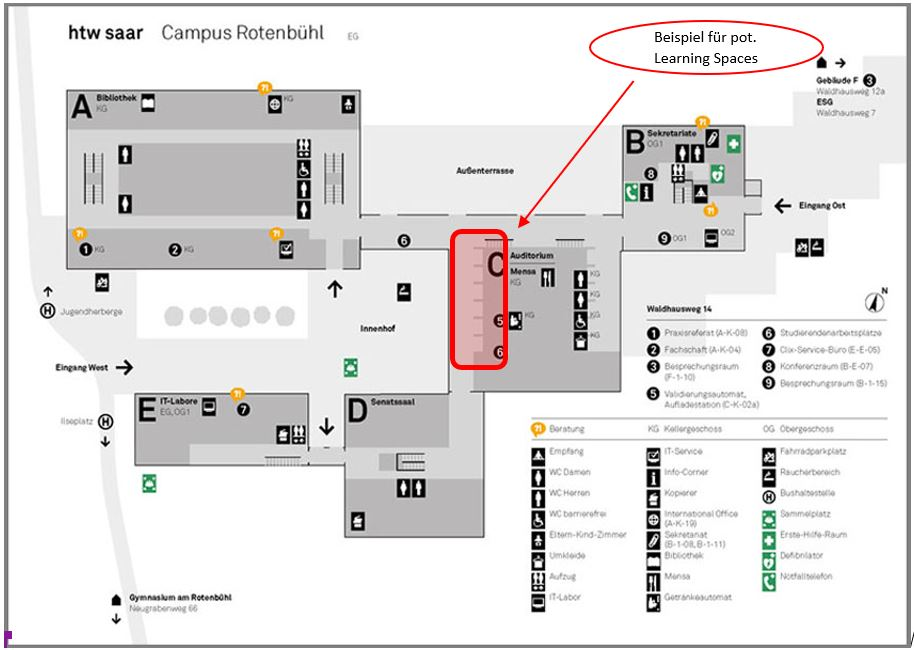
\includegraphics[width=1\textwidth]{Bilder/OrtSpaces}\\
\end{figure}

\newpage
\subsection{Betriebsbedingungen}
Die Betriebsbedingungen für die Software zur Raumbuchung bleiben in absehbarer Zukunft die gleichen. Abgesehen von Wartungen herrscht ein Dauerbetrieb der Anwendung, sodass Nutzer jederzeit die Möglichkeit haben Räume für sich zu reservieren. Eine spezifische tägliche Betriebszeit entfällt damit. Das System bedarf keiner ständigen Beobachtung durch einen Administrator und läuft somit prinzipiell unbeaufsichtigt. Die maximale Anzahl an Benutzern ist tendenziell unbegrenzt, sollte im Regelfall allerdings nicht die Anahl an Studierenden und Mitarbeiter der htw am Campus Rothenbühl übersteigen. Zudem kann davon ausgegangen werden, dass der sich der jeweilige Zeitpunkt der Nutzung der Software über den Tag hinweg verteilt, sodass es als eher unwahrscheinlich anzusehen ist, dass es zu Ballungen und Überlastungen des Systems kommt.
 
\newpage

\section{Funktionen}
Dieses Kapitel enthält die Grundlegenden Funktionen und Bestandteile des Programmes. Es folgen:\\
- Klassendiagramm\\
- Aktivitätsdiagramm\\
- Use-CaseDiagramm\\ 

\subsection{Klassendiagramm}
Das Klassendiagramm verfügt über die Generalisierungsklasse User, welche alle allgemeinen Attribute eines Nutzers enthält. Die Klasse User teilt sich in die Spezialisierungsklassen Student, Dozent und Mitarbeiter auf und vererbt sinngemäß die allgemeinen Attribute an die Spezialisierungsklassen. Die speziellen Attribute sind in der jeweiligen Klasse hinterlegt. Zudem ist die Klasse Admin Teil der User-Klasse. Hierbei muss ein Admin immer existieren, der das System verwaltet. Da ein Admin auch ein User ist, muss folglich auch mindestens ein User existieren. Es können aber auch mehrere User und mehrere Admins gleichzeitig existieren. Ein Admin verfügt über den Zugriff auf alle Methoden des Systems.\\
Einem User kann immer genau ein Account zugeordnet werden. Hierbei besteht die Beziehung, dass wenn ein User nicht existiert, dann existiert auch sein dazugehöriger Account nicht. Umgekehrt kann das sehr wohl der Fall sein. Mit Hilfe der in der User-Klasse hinterlegten Attribute, kann man seinen Account im System anmelden (einloggen) bzw. abmelden (ausloggen).\\
Die Klasse Buchung enthält alle Informationen über eine Buchung. Hierbei kann ein Account mehrere Buchungen verfügen, aber eine Buchung ist immer genau einem Account zugeordnet. Eine Buchung kann Buchung kann Buchungen anzeigen, Räume buche und stornieren sowie einen Timeslot auswählen. Da an eine Buchung bestimmt Restriktion geknüpft sind, gibt es einen Buchungsstatus, der ausgibt, ob meine Buchung noch angefragt wird oder bereits eine Bestätigung oder Absage erteilt wurde. Eine Buchung enthält genau einen gebuchten Raum und einen gebuchten Timeslot. Die Klasse Space enthält Information über den Raum wie die RaumID, Platzanzahl und PC-Anzahl. Die Klasse Timeslot enthält die Informationen zum gewählten Datum, Uhrzeit und der Dauer.
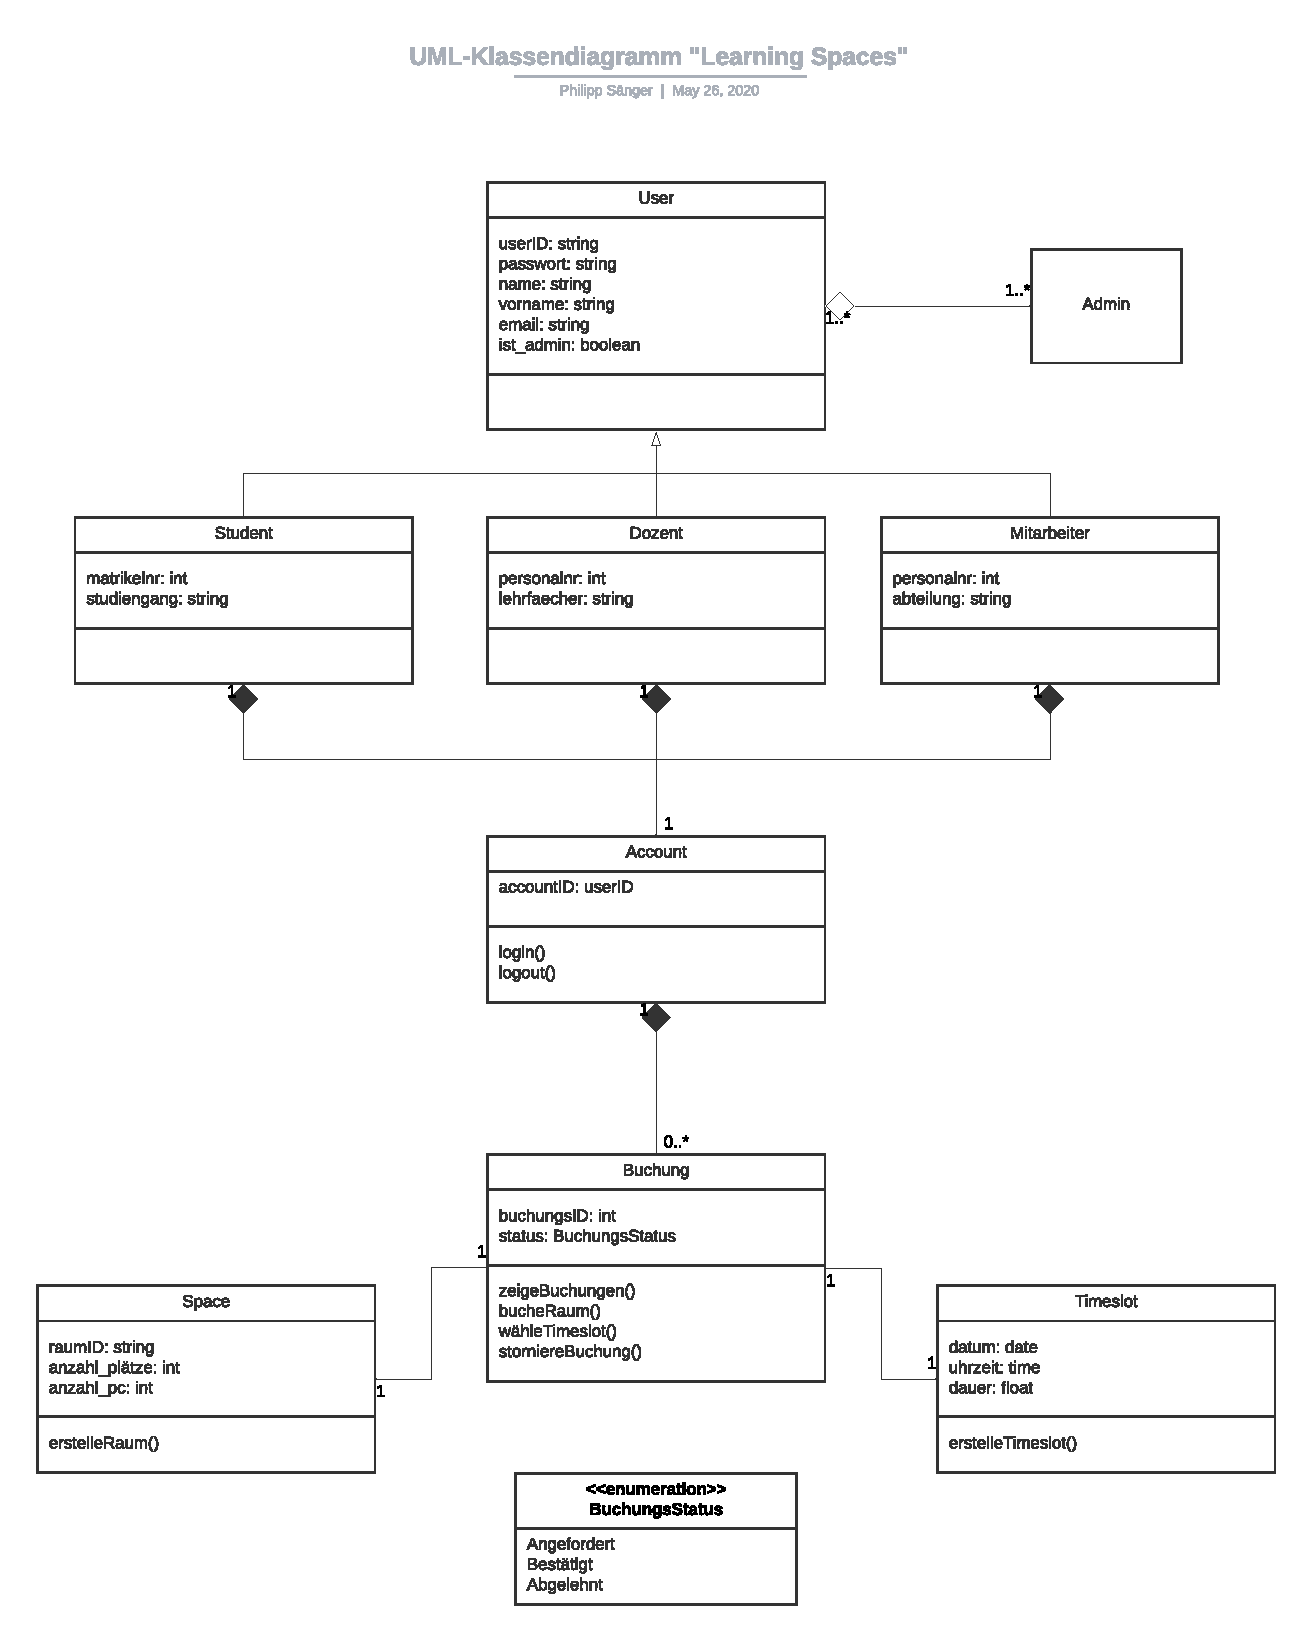
\includepdf{PDF/Klassendiagramm}\label{Klassendiagramm}

\subsection{Aktivitätsdiagramm}
Im Aktivitätsdiagramm wird die Programmlogik abgebildet. Zur Buchung eines Raumes wird nach Aufruf der Website eine Anmeldung verlangt. Ist diese erfolgt, kann ein Zeitslot gewählt werden. Die Räume werden angezeigt. Ist kein Raum zu diesem Zeitslot verfügbar, kann ein neuer Zeitslot gewählt werden. Ist ein Raum verfügbar, kann dieser ausgewählt und die Buchung bestätigt werden. Der Vorgang wird mit dem Abmelden des Benutzers abgeschlossen.\\

\begin{figure}[h]
\begin{center}
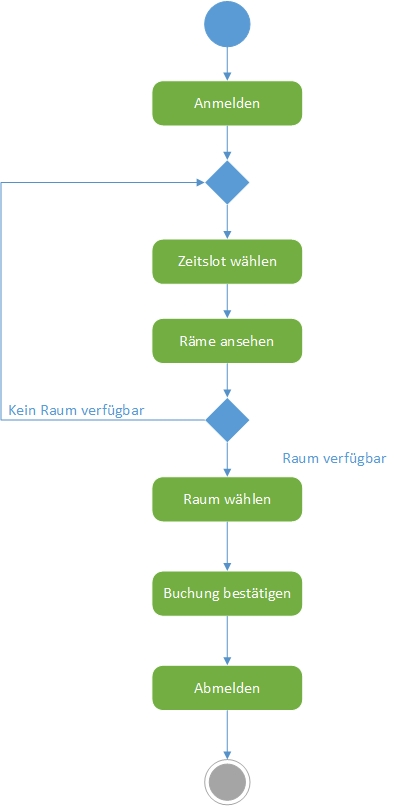
\includegraphics[width=0.6\textwidth]{Bilder/Aktivitaetsdiagramm}\label{Aktivitaetsdiagramm}
\end{center}
\end{figure}
%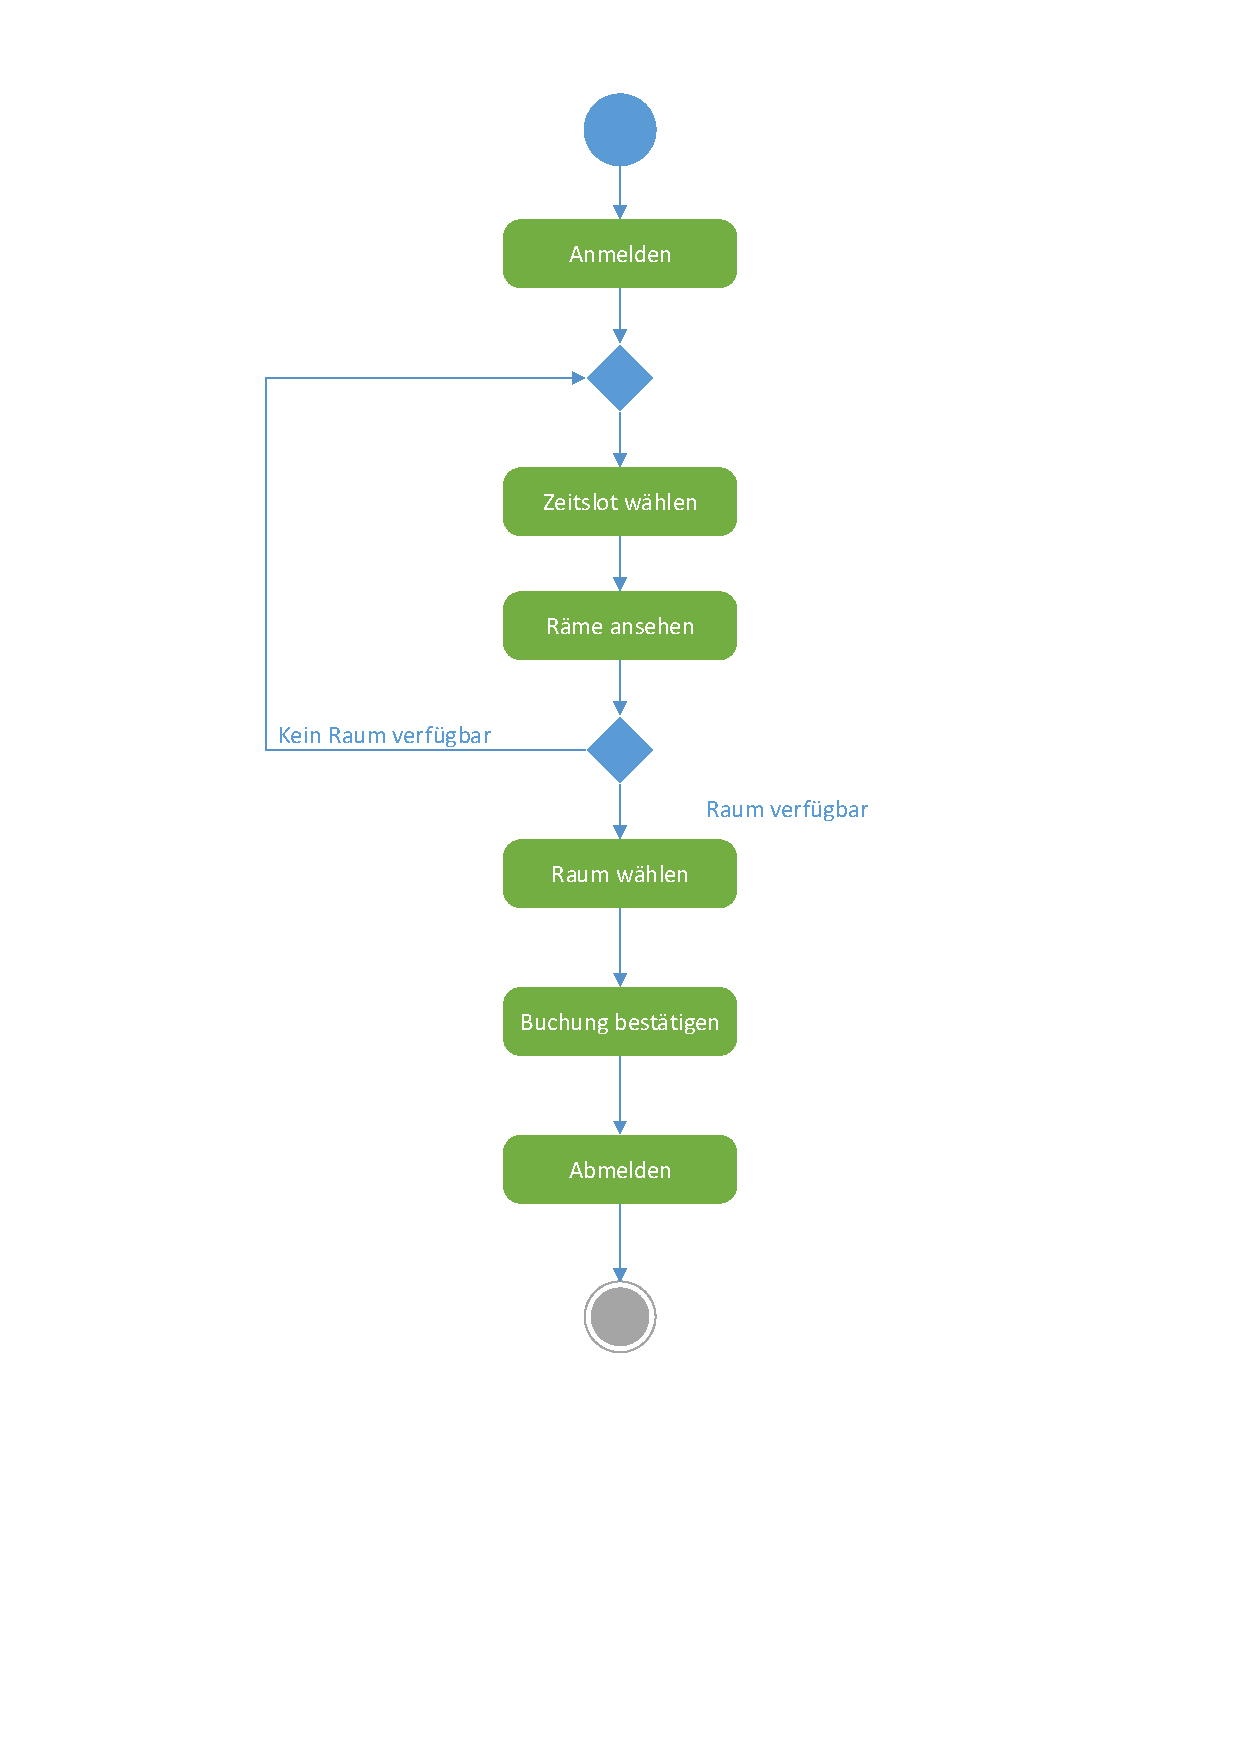
\includepdf[pages=1,scale=1]{PDF/Aktivitaetsdiagramm}\label{Flussdiagramm}

\subsection{Use-Case-Diagramm}
Für das Projekt Learning Spaces wurde im Vorfeld ein Use Case Diagramm erstellt, um die verschiedenen Anwendungsfälle des Systems zu visualisieren. Das Learning Spaces System steht dabei mit zwei Akteuren, dem User und dem Admin, in Kontakt. Für den Anwendungsfall Login kann mit einem weiteren System der htw über eine Schnittstelle per Lightweight Directory Access Protocol (LDAP) kommuniziert werden, um die bestehenden htw Accounts für den Login in das Learning Spaces System zu nutzen. Des Weiteren stehen dem einfachen Nutzer die Anwendungen Raum buchen und Buchung stornieren zur Verfügung. Gleiches gilt für den Admin, mit dem Unterschied, dass dieser mehrere Räume gleichzeitig Buchen und stornieren kann. Ebenfalls exklusiv steht dem Admin die Anwendung Accounts erstellen/löschen zur Verfügung.\\

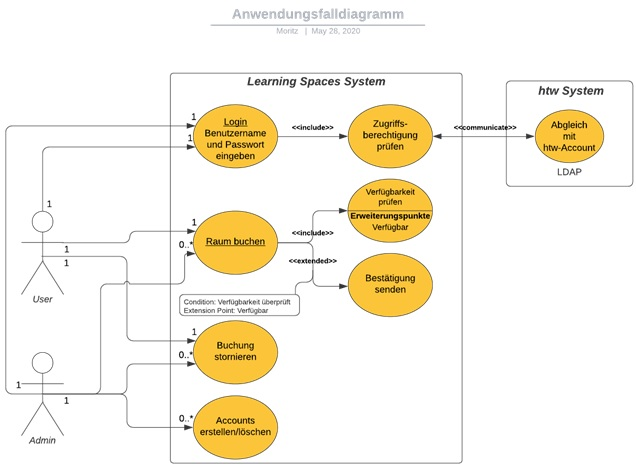
\includegraphics{Bilder/UseCaseDiagramm}\label{UseCase}\\

\newpage

\section{Nichtfunktionale Anforderungen}
Zu den wichtigsten Qualitätsanforderungen der Applikation "Learning Spaces" zählen die Benutzbarkeit und die Übertragbarkeit. Die Anwendung soll eine möglichst einfache Handhabung aufweisen, denn durch eine intuitive Menüführung, die für jedermann verständlich ist, wird eine zusätzliche Einweisung in das System nicht benötigt. Aufgrund der bestehenden IT-Infrastruktur der HTW Saar soll die App kompatibel mit den bereits implementierten Schnittstellen sein. Zur einfachen Einbindung soll die App mit dem django webframework umgesetzt werden und das Layout soll an die Coperate Identity angepasst sein.\\ 
Etwas weniger wichtig, jedoch auch zu berücksichtigen sind die Aspekte Zuverlässigkeit, Effizienz sowie Änderbarkeit des Systems. Um die Zuverlässigkeit der Anwendung zu erhöhen, sollte eine Problembehandlung integriert werden, wodurch Eingabefehler durch einen Benutzer vermieden werden. Des Weiteren werden kontinuierlich Testreihen durchgeführt, ehe das Programm freigegeben wird, um ein fehlerfreies System zu Verfügung zu stellen. Weiterhin sollen die Funktionen nicht irgendwie, sondern möglichst schlank umgesetzt werden. Denn ein großer Quellcode führt natürlich auch zu einem größeren Ressourcenverbrauch und einer höheren Reaktionszeit, wodurch die Effizienz des arbeitenden Systems gestört wird. Abschließend soll eine Änderbarkeit der App jederzeit ermöglicht werden. Hierzu wird auf die Verwendung von Git und GitHub, einem Versionskontrollsystem, gesetzt. Um die nachträgliche Veränderung des Programms durch externe Personen zu vereinfachen, wird der Quellcode mit verständlichen Kommentaren versehen, sodass leicht zu erkennen ist, welche Funktionen die jeweiligen Programmierungsabschnitte innehaben.\\

\section{Benutzeroberfläche}
Analog zum Dashboard soll hier die Übersichtlichkeit und die Einfachheit der Bedienung im Vordergrund stehen. Farben und Texturen sollen sparsam verwendet, optisch aufeinander abgestimmt werden und der Corporate Identity der HTWsaar entsprechen. Eine konsistente Bedienerführung, im Sinne von gleichartigen Bedienelementen als auch überschaubare Informationseinheiten sollen den gesamten Aufbau des Programms durchziehen und die Bedienung damit ebenfalls erleichtern.\\ 

Der erste Bildschirm, der beim Aufruf der Website erscheint, ist der Anmeldevorgang. Hier muss im ersten Schritt ausgewählt werden, um welche Person (Student/Dozent/Mitarbeiter) es sich handelt.\\

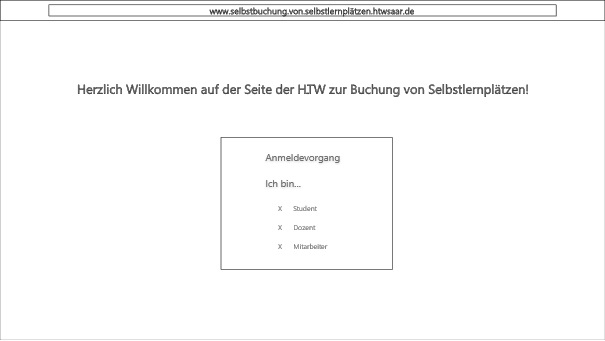
\includegraphics{Bilder/UI1}\label{UI_1}\\

Im Nachfolgenden Schritt kann man sich, soweit bereits ein Account vorhanden ist, auf der Website anmelden. Alternativ kann man über den Reiter „Registrieren“ einen neuen Account erstellen.\\

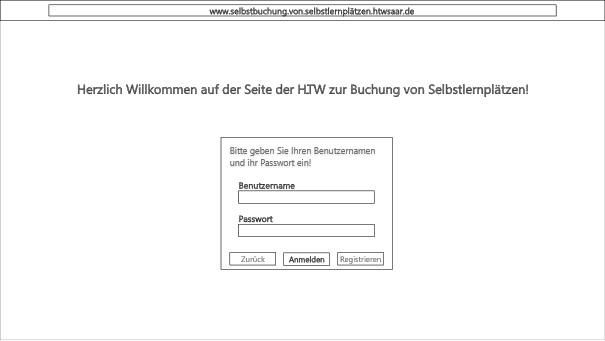
\includegraphics{Bilder/UI2}\label{UI_2}\\

Sollte der Anmeldevorgang gescheitert sein, beispielsweise aus dem Grund eines Tippfehlers oder weil noch kein Account erstellt wurde, so erscheint eine entsprechende Fehlermeldung und die Person wird auf die erste Anmeldeseite zurückgeführt.\\

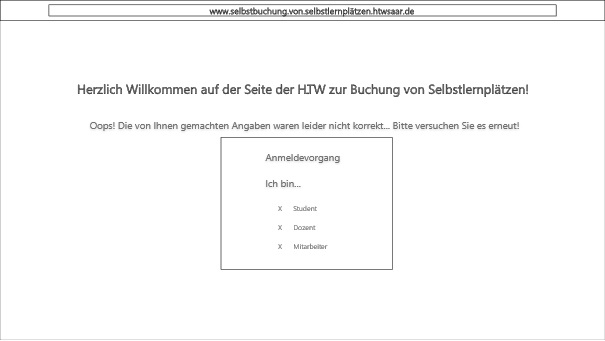
\includegraphics{Bilder/UI3}\label{UI_3}\\

Nach dem Anmeldevorgang gelangt man zur Startseite. Hier erhält man einen ersten Überblick über den Aufbau der Website und es wird eine „Begrüßungsnachricht“ angezeigt, worin unter anderem erklärt wird, unter welchen Bedingungen Raumbuchungen vorgenommen werden können.\\

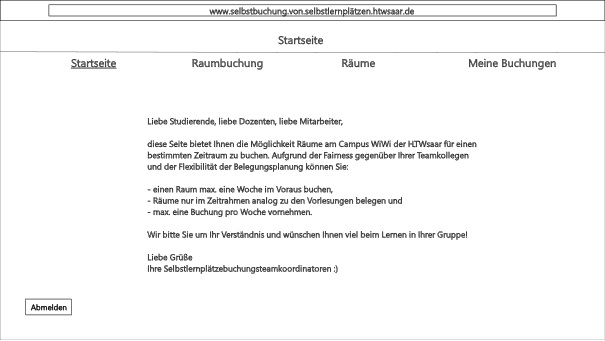
\includegraphics{Bilder/UI4}\label{UI_4}\\

Über eine überschaubare Anzahl an Reitern kann durch die Seite navigiert werden. Nach heutigem Stand kann über den Reiter „Raumbuchung“ ein Raum gebucht werden.\\

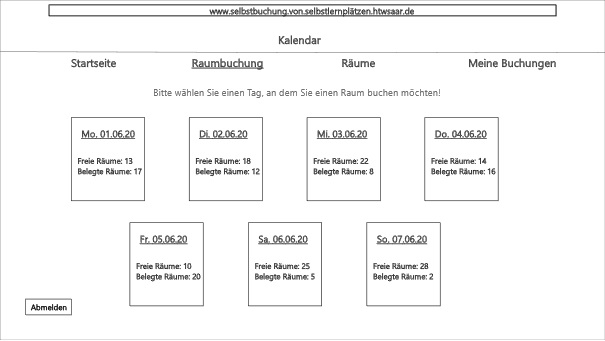
\includegraphics{Bilder/UI5}\label{UI_5}\\

Unter dem Reiter „Raumbuchung“ kann einer der folgenden sieben Wochentage ausgewählt werden. Hierbei soll direkt ein aktueller Stand ersichtlich sein, wie viele Räume bereits belegt und wie viele noch frei sind.\\

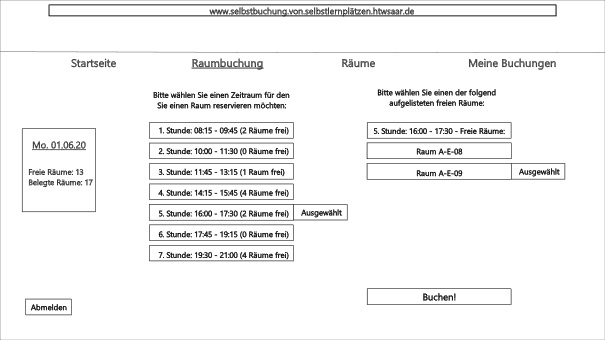
\includegraphics{Bilder/UI6}\label{UI_6}\\

Sobald man sich für einen Tag entschieden hat, so muss sich entscheiden, für welche Stunde man einen Raum buchen möchte. Auch hierbei sollte erneut direkt ersichtlich sein, zu welcher Stunde wie viele Räum noch frei bzw. belegt sind.\\ 
Nach dem Auswählen der Stunde werden folglich alle Räume aufgelistet, die zu dieser Stunde noch frei sind.\\
Erst danach soll weiter unter der „Buchen“-Button erscheinen, über dessen Anklicken verbindlich ein Raum reserviert wird.\\

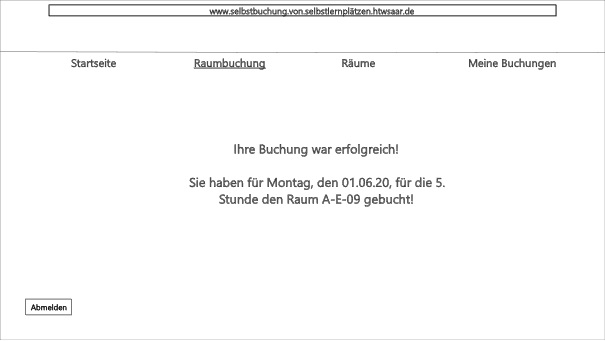
\includegraphics{Bilder/UI7}\label{UI_7}\\

Eine passende Ereignismeldung bestätigt die Raumbelegung.\\
Über den Reiter „Räume“ soll aufgeführt werden, über welche technische Mittel ein Raum verfügt (Beamer, Tafel, …)\\

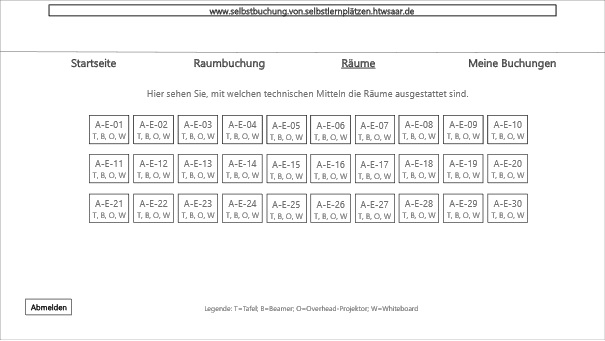
\includegraphics{Bilder/UI8}\label{UI_8}\\

Über den Reiter „Meine Buchungen“ kann eingesehen werden, welche Buchung unter dem jeweiligen Account bereits vorgenommen wurde.\\
Der Abmeldebutton führt zum Logout.\\

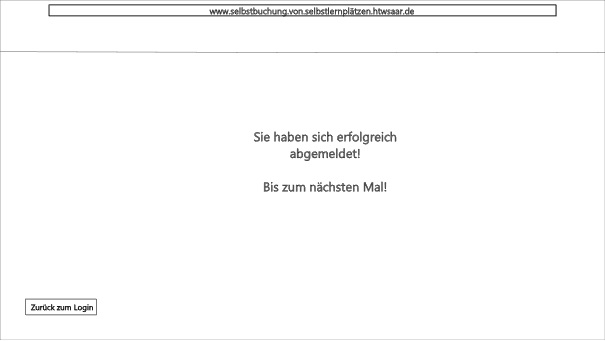
\includegraphics{Bilder/UI9}\label{UI_9}\\

\section{Projektablaufplan}
Das Projekt gliedert sich in drei Phasen, welche jeweils mit einem Meilenstein abgeschlossen werden. Zu Beginn erfolgt über vier Wochen in der Analysephase die Einarbeitung in das Projekt sowie die grundsätzliche Konzeption des Aufbaues der Software. Abgeschlossen wird diese erste Phase mit dem Meilenstein Abgabe des Pflichtenheftes. Anschließend folgt die neunwöchige Implementierungsphase, in der die zugrundeliegenden Rahmenbedingungen definiert werden und die Implementierung von Klassen und Funktionen auf codeebene erfolgt. In der Implementierungsphase werden etappenweise Sprint logs durchgeführt, welche von wöchentlichen Scrum Meetings begleitet werden. Diese Phase wird mit dem zweiten Meilenstein Veröffentlichung Alpha Version beendet. Abschließend folgt die dritte Projektphase Release in, der über vier Wochen, die Alpha Version getestet wird und an offene Kundenwünsche angepasst wird. Final erfolgt der Projektabschluss mit Realisierung des dritten Meilensteins, dem Launch der Applikation. Das gesamte Projekt umfasst somit einen Zeitraum von 17 Wochen.\\

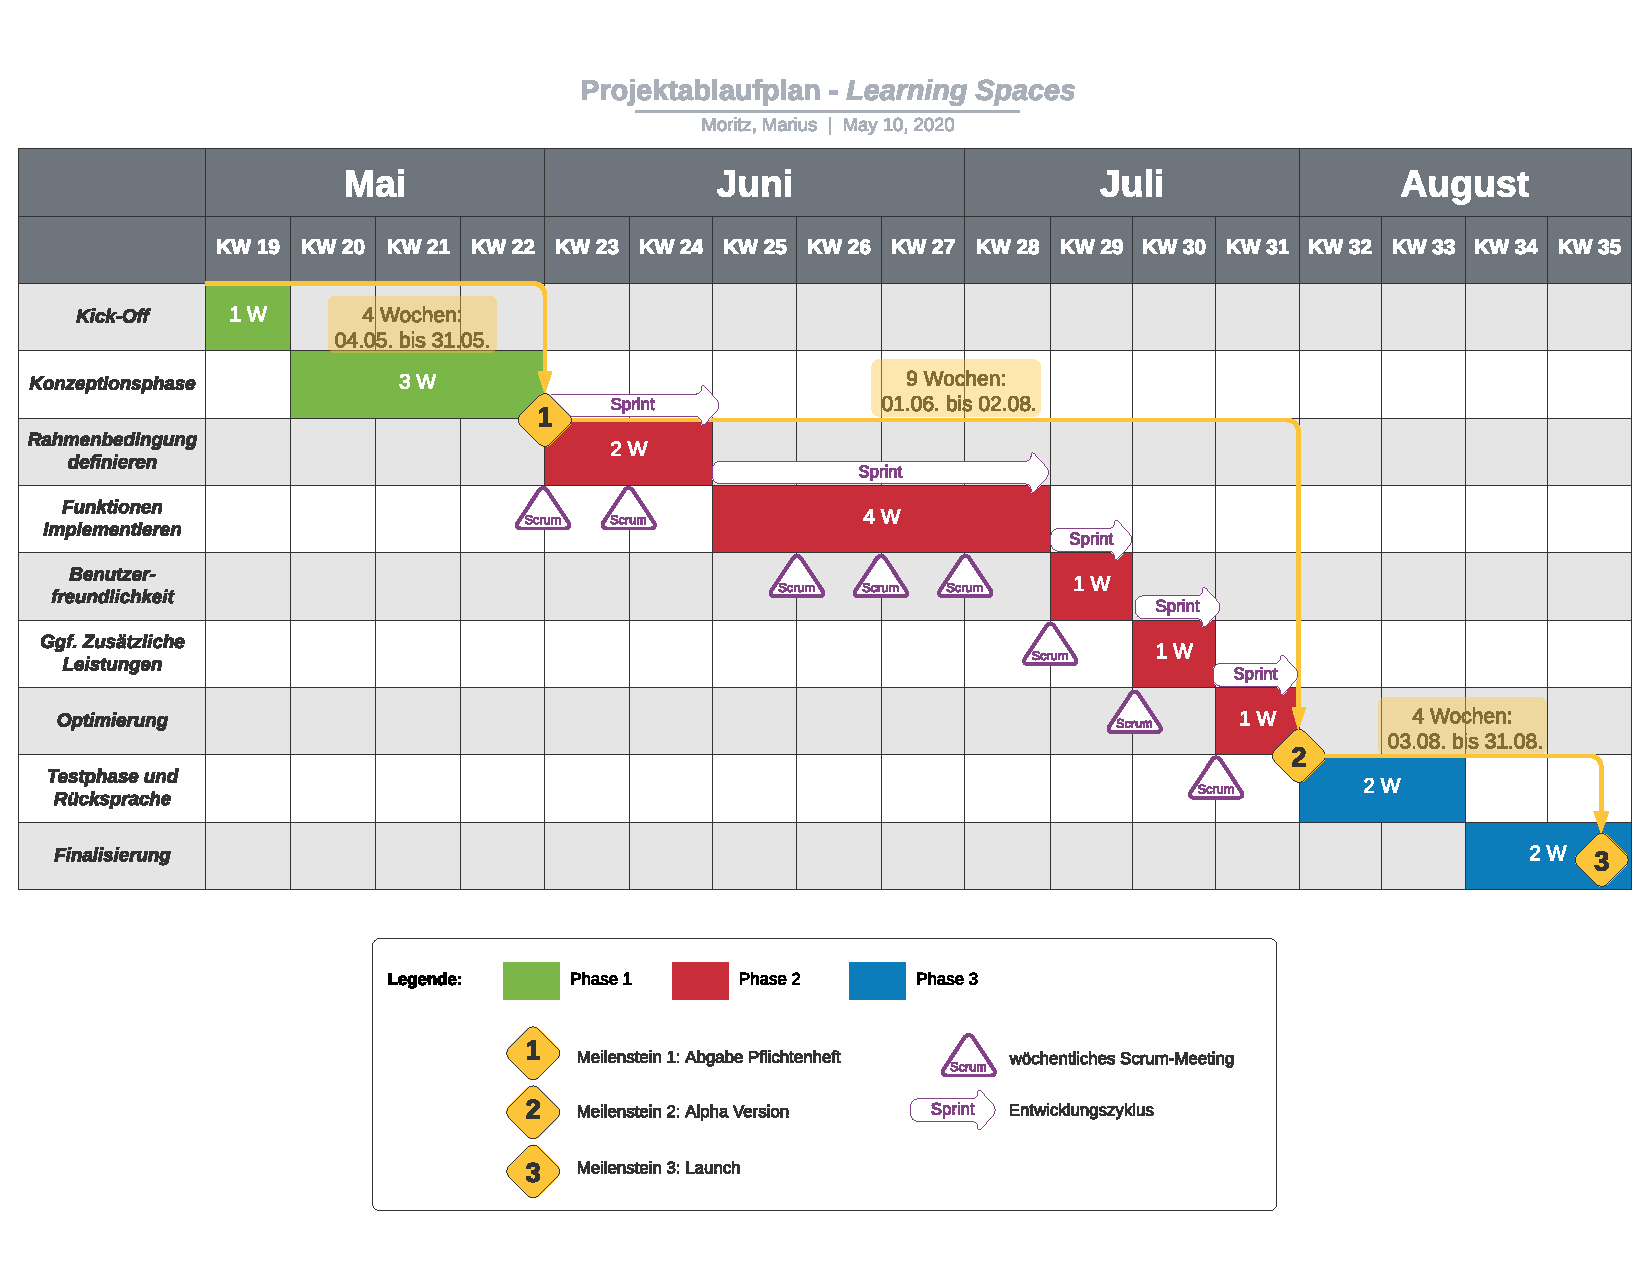
\includepdf[landscape,pages=1,scale=1]{PDF/Projektablaufplan}\label{Projektablaufplan}

\end{document}